Una LookUp Table, o LUT, en términos generales es básicamente una tabla que determina cuál es la salida para cualquier entrada dada. En el contexto de la lógica combinacional, es la tabla de verdad. Esta tabla de verdad define efectivamente cómo se comporta su lógica combinatoria.

En otras palabras, cualquier comportamiento que obtenga al interconectar cualquier número de compuertas (como AND, NOR, etc.), sin rutas de retroalimentación (para garantizar que no tenga estado), puede implementarse mediante una LUT.

Una LUT generalmente se construye a partir de Bits SRAM para contener la máscara LUT de la memoria de configuración (CRAM) y un conjunto de multiplexores para seleccionar el bit de CRAM que es conducido a la salida. Para implementar una LUT de entrada k (LUTk), una LUT que puede implementar cualquier función de k entradas necesita 2\textsuperscript{k} bits SRAM y un multiplexor 2\textsuperscript{k}:1. La Figura \ref{altera_luts_1} muestra una LUT4, que consta de 16 bits de SRAM y un multiplexor 16:1 implementado como un árbol de multiplexores 2:1. La LUT4 puede implementar cualquier función de 4 entradas (A, B, C, D) configurando el valor apropiado en la máscara LUT. Para simplificar la LUT4 en la Figura \ref{altera_luts_1}, también se puede construir a partir de dos LUT3 conectadas por un multiplexor 2:1.

\begin{figure}[H]
	\centering
	\includegraphics[width=1 \textwidth]{img/altera_luts_1.png}
	\caption{Construyendo una LUT}
	\label{altera_luts_1}
\end{figure}


De manera similar, las LUT más grandes se pueden construir a partir de las más pequeñas ~\cite{alteraLUTs}, como se muestra en la Figura \ref{altera_luts_2}. Por ejemplo, se puede construir una LUT5 con dos LUT4 y un multiplexor, mientras que un LUT6 se puede construir con dos LUT5 y un multiplexor. Técnicamente, lo importante es el número total de bits CRAM en la LUT y que se utilizan para implementar una función arbitraria de seis entradas.


\begin{figure}[H]
	\centering
	\includegraphics[width=0.6 \textwidth]{img/altera_luts_2.png}
	\caption{Composición de LUTs más grandes a partir de LUTs más pequeñas}
	\label{altera_luts_2}
\end{figure}

Teniendo esto en cuenta, y sabiendo que MODNET permite realizar una inyección por cada LUT dentro del circuito, podemos transformar de forma iterativa cada una de las LUTs existentes para convertirlas en LUT2, y así conseguir un aumento exponencial de inyecciones mayor al anteriormente conseguido, como se observa en la figura \ref{lut4_to_lut2}.

\begin{figure}[t]
	\centering
	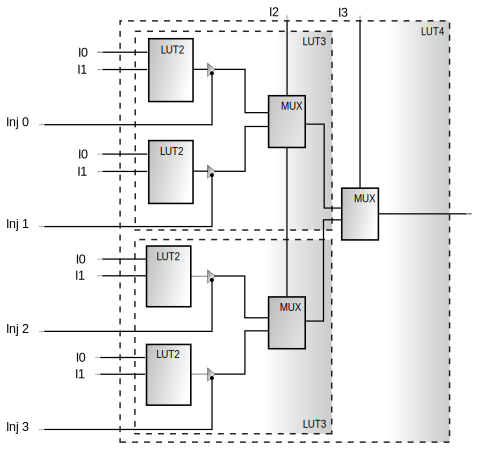
\includegraphics[width=0.7 \textwidth]{img/Lut4_IN_LUT2.pdf}
	\caption{Implementación de una a LUT4 con 4 LUT2s y 3 multiplexores o 2 LUT3s y 2 multiplexers}
	\label{lut4_to_lut2}
\end{figure}